%
%-----------------------------------
\section{Stochastic evolution}
\label{sec:stochastic-evolution}
%-----------------------------------
%

Let us consider an atom at $ \mathbf{r_0} $ and with the velocity $ \mathbf{v_0} $ in the presence of laser beams and a quadrupole magnetic field. After a period $ \delta t $, this atom can absorb a photon with momentum $ \hbar \mathbf{k_j} $ and then emit a photon with momentum $ \hbar |\mathbf{k}_j| \mathbf{\hat{u}} $, where $ \mathbf{\hat{u}} $ is an uniform unit random vector and $ \mathbf{k}_j $ is the wave vector of the $j$-th laser beam. Also, since there is a magnetic field gradient, a magnetic force acts on the atom as discussed in section \ref{sec:magnetic-force} that yields a position-dependent acceleration $ \mathbf{a}_{B}(\mathbf{r_0}) $. Therefore, the atom's velocity $ \mathbf{v}_i $ and position $ \mathbf{r}_i $ at instant $ i \delta t $, where $ i = 0, 1, \cdots $, are
\begin{equation}
    \mathbf{v}_i = \left\{ \begin{array}{lr}
        \mathbf{v}_{i - 1} + \hbar \frac{|\mathbf{k}_j|}{m}(\mathbf{\hat{k}}_j + \mathbf{\hat{u}}) + (\mathbf{a}_B(\mathbf{r}_{i - 1})- g \mathbf{\hat{z}}) \delta t, & \textrm{with probability}\ P_{i}
        \\
        \mathbf{v}_{i - 1} + (\mathbf{a}_B(\mathbf{r}_{i - 1})- g \mathbf{\hat{z}}) \delta t, & \textrm{with probability}\ 1 - P_{i}
        \end{array} \right.
        \label{eq:atom-velocity-iteration}
\end{equation}
and
\begin{equation}
    \mathbf{r}_i = \mathbf{r}_{i - 1} + \mathbf{v}_{i}\delta t + (\mathbf{a}_B(\mathbf{r}_{i - 1}) - g \mathbf{\hat{z}}) \delta t^2 / 2,
    \label{eq:atom-position-iteration}
\end{equation}
where $ P_{i} \equiv P(\mathbf{r} = \mathbf{r}_i, \mathbf{v} = \mathbf{v}_i | \mathbf{r}_{i - 1}, \mathbf{v}_{i - 1}) $ is the probability of happing a scattering event also known as \textbf{transition probability}. Since $ P_i $ is a conditional probability that depends only on the previous atom state, the dynamics is then a \textbf{memoryless stochastic process}, also known as \textbf{Markov chain}. The goal is to sample trajectories $ \mathbf{r}(t) $ and velocities $ \mathbf{v}(t) $ in order to estimate the probability distributions of the atom's position and velocity. To perform this, we iterate the equations (\ref{eq:atom-velocity-iteration}) and (\ref{eq:atom-position-iteration}) and then fill up histograms.


%-----------------------------------
\subsection{Equilibrium}
\label{sec:equilibrium}
%-----------------------------------

Let us consider the vector $ \rho(t) = \rho(i\delta) = \rho_i $ in which each component is the probability of an atom being at specific position $ \mathbf{r} = (x, y, z) $ with a specific velocity $ \mathbf{v} = (v_x, v_y, v_z) $ at a instant $ t $.
We shall call this vector as \textbf{atom state}. Although position and velocity are continuous variables, we must discrete both to perform a feasible computation. If we consider $ N $ possible values for $ x $, $ y $, $ z $, $ v_x $, $ v_y $, and $ v_z $, the dimension of the vector $ \rho_i $ is $ N^6 $, which means that the dimension of the problem escalates very quickly. Since the probabilities related to each component of position ($ x $, $ y $, and $ z $) and velocity ($ v_x $, $ v_y $, and $ v_z $) are independent, we only need the marginal distributions so that the total dimension will be reduced to $ 6N $. It is also possible to represent the transition probabilities $ P_i $ in the same vector space as a matrix $ \mathbf{P} $ of which each element is $ P(\mathbf{r} = \mathbf{r}_i, \mathbf{v} = \mathbf{v}_i | \mathbf{r}_{i - 1}, \mathbf{v}_{i - 1}) $\footnote{We are assuming that $ \mathbf{r} $ and $ \mathbf{v} $ are discrete variables}. Therefore, after $ n $ iterations, the atom state will be \cite[Section~23.2]{wasserman2004all}
\begin{equation}
    \rho_n =  \rho_0 \underbrace{(\mathbf{P} \times \mathbf{P} \times \cdots \times \mathbf{P})}_{\textrm{mutiply the matrix $n$ times}} = \rho_0 \mathbf{P}^n,
\end{equation}
where $ \rho_0 $ is the initial atom state given by a deterministic vector since we set the initial atom's position and velocity. We expect that $ \rho $ be constant after a sufficient number of iterations, which it is observed experimentally. Thus, $ \rho = \rho\mathbf{P} $ for large enough $ n $. In this case, we say that $ \rho $ is \textbf{stationary}. The purpose of the simulation is to estimate the atom state $ \rho $. In order to obtain proper samples of $ \rho $, we only save $ \mathbf{r} $ and $ \mathbf{v} $ after a number of iterations.

%-----------------------------------
\subsection{Magnetic field basis}
\label{sec:magnetic-field-basis}
%-----------------------------------

\begin{wrapfigure}{l}{0.4\textwidth}
    \centering
    \vspace{-10px}
    \caption{Magnetic field basis}
    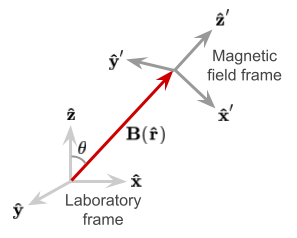
\includegraphics[width=0.3\textwidth]{USPSC-img/polarization_basis.png}
    \legend{basis $ A' = \{\mathbf{\hat{x}}', \mathbf{\hat{y}}', \mathbf{\hat{z}}'\} $ of the magnetic field frame in relation to the basis $ A = \{\mathbf{\hat{x}}, \mathbf{\hat{y}}, \mathbf{\hat{z}}\} $ of the laboratory frame. \\ Source: author}
    \label{fig:magnetic-field-basis}
    \vspace{0px}
\end{wrapfigure}

We shall consider the assumptions introduced in section \ref{sec:MOT-force}, which simplifies a four-level system in three independent two-level systems associated with the polarizations $ \sigma_{\pm} $ and $ \pi $. In this condition, for each laser beam, there are three possible transitions, each one with its scattering rate $ R_{i,j,l} $, where $ l \in \{\sigma_{+}, \sigma_{-}, \pi \} $. Initially, we define the laser polarizations on the basis $ \mathbf{B} = \{\hat{\sigma}_{+}, \hat{\sigma}_{-}, \hat{\pi} \} $ so that
\begin{equation}
    \hat{\sigma}_+ = \frac{\mathbf{\hat{x}} + i\mathbf{\hat{y}}}{\sqrt{2}},\ \ \hat{\sigma}_- = \frac{\mathbf{\hat{x}} - i\mathbf{\hat{y}}}{\sqrt{2}},\ \ \hat{\pi} = \mathbf{\hat{z}},
\end{equation}
where $ A = \{\mathbf{\hat{x}}, \mathbf{\hat{y}}, \mathbf{\hat{z}}\} $ is the basis of the laboratory frame. To account the magnetic field $ \mathbf{B} $ effect in $ R_{i,j,l} $, we must analyse the magnetic field in a frame that defines the quantization axis parallel to $ \mathbf{B} $. Let us consider the basis $ A' = \{\mathbf{\hat{x}}', \mathbf{\hat{y}}', \mathbf{\hat{z}}'\} $ in the the magnetic field frame as illustrated in figure \ref{fig:magnetic-field-basis}.

The polarization basis $ \mathbf{B}' = \{\hat{\sigma}_{+}', \hat{\sigma}_{-}', \hat{\pi}' \} $ in the magnetic field frame is given by
\begin{equation}
    \hat{\sigma}_+' = \frac{\mathbf{\hat{x}'} + i\mathbf{\hat{y}}'}{\sqrt{2}},\ \ \hat{\sigma}_-' = \frac{\mathbf{\hat{x}'} - i\mathbf{\hat{y}}'}{\sqrt{2}},\ \ \hat{\pi}' = \mathbf{\hat{z}}' \| \mathbf{B}.
\end{equation}

Let us consider the polarization vector $ \hat{\epsilon}_j $ of the $ j $-th laser beam defined as $ [\hat{\epsilon}_j]_B $ on the laboratory basis $ B $. Its components on the basis $ B' $ is given by $ [\hat{\epsilon}_j]_B' = M [\hat{\epsilon}_j]_B $, where $ M $ is the change-of-basis matrix. We must consider two other change-of-basis matrices to obtain $ M $. The first one is the matrix $ M' $ that change a polarization basis such as $ B $ to a Cartesian basis such as $ A $. The second one is the rotation matrix $ R(\theta) $. Thus, the change-of-basis $ M $ is given by
\begin{equation}
    M = (M')^{\dagger}R(\theta)M',\ \ (M')^{\dagger} = ((M')^*)^T = (M')^{-1},
\end{equation}
where
\begin{equation}
    M' = \left[ \begin{matrix}
        1/\sqrt{2} & 1/\sqrt{2} & 0 \\
        -i/\sqrt{2} & i/\sqrt{2} & 0 \\
        0 & 0 & 1
    \end{matrix} \right],\ \
    R(\theta) = \left[ \begin{matrix}
        1 & 0 & 0 \\
        0 & \cos(\theta) & -\sin(\theta) \\
        0 & \sin(\theta) & \cos(\theta)
    \end{matrix} \right].
\end{equation}

%-----------------------------------
\subsection{Transition probabilities}
\label{sec:transition-probabilities}
%-----------------------------------

The scattering rate $ R_{i,j,l} $ is essentially the time derivative of the probability of scattering a photon of the $j$-th laser beam due to transition $ l $. Hence, the probability $ P_{i,j,l} $ of happing a scattering event during a time interval $ \delta t $ is given by
\begin{equation}
    R_{i,j,l} = \frac{\partial P_{i,j,l}}{\partial t} \Rightarrow P_{i,j,l} \simeq R_{i,j,l} \delta t.
\end{equation}
The probability of a photon from the $j$-th laser beam having the polarization $ l $ is $ \left| \braket{\hat{\epsilon}_j|\mathbf{\hat{e}}_l} \right| $, where $ \mathbf{\hat{e}}_l \in B' $. Thus, the transition probability $ P_{i,j} $ is given by
\begin{equation}
    P_{i,j} = \sum_{l} \left| \braket{\hat{\epsilon}_j|\mathbf{\hat{e}}_l} \right| P_{i,j,k} =  \sum_{l} \left| \braket{\hat{\epsilon}_j|\mathbf{\hat{e}}_l} \right| R_{i,j,l} \delta t.
\end{equation}
From equation (\ref{eq:radiation-pressure-force-2}), we have
\begin{equation}
    R_{i,j,l} = \frac{\Gamma}{2}\frac{s(\mathbf{r})}{1 + s(\mathbf{r}) + (2\Delta_l / \Gamma)^2},\ \ s(\mathbf{r}) = \exp\left[\ -\frac{2(x^2 + y^2)}{w^2} \right],\ \ \Delta_l = \delta + \delta_Z^{(l)} + \delta_D,
\end{equation}
where $ w $ is the waist of the $ j $-th laser beam, $ \delta $ is the laser detuning, $ \delta_Z^{(l)} $ is the Zeeman shift due to the $ l $ transition given by equation (\ref{eq:Zeeman-shift}), and $ \delta_D = - \mathbf{k} \cdot \mathbf{v}_{i - 1} $ is the Doppler shift. To increase accuracy, we are taking into account the Gaussian profile of the laser beams in $ s(\mathbf{r}) $.
